\section{Problem formulation}

\subsection{Trilateration}\label[secc]{trilat}
Given $n\geq 3$ agents located at positions $\mathbf{x}_{a}\in\mathbb{R}^{2},\; 0\leq a<n$ the location 
of an entity, denoted by $\mathbf{y}\in\mathbb{R}^{2}$, can be determined as follows:
\begin{enumerate}
  \item The entity broadcasts signal and starts a timer at $t_{0}$.
  \item Agents at $\mathbf{x}_{a}$ receives broadcasted signal and immediately responds with a packet containing $\mathbf{x}_{a}$.
  \item When receiving the packet from agent ${a}$, the entity stores the time of reception in a variable $t_{1, a}$.
  \item When at least 3 agents have responded, the entity calculates the distance
  from itself to agent $a$: $d_{a} = \frac{1}{2}c(t_{1, a} - t_{0})$, where $c$ is the speed of light. The factor $\frac{1}{2}$ is due to the signal traveling
  two times the distance between the entity and agent $a$ (the ping travels from the entity to the agent, and the packet
  sent by the agent travels back again).
  \item Based on the distances, $d_{a}$, and the positions of the agents, $\mathbf{x}_{a}$, the entity can
  determine its position by calculating the point where circles centered at $\mathbf{x}_{a}$ with radii $d_{a}$ intersect.
\end{enumerate}
\figref{trilat_example} shows how the position of an entity can be determined from the known positions of 3 agents.
\begin{figure}[H]
  \centering
  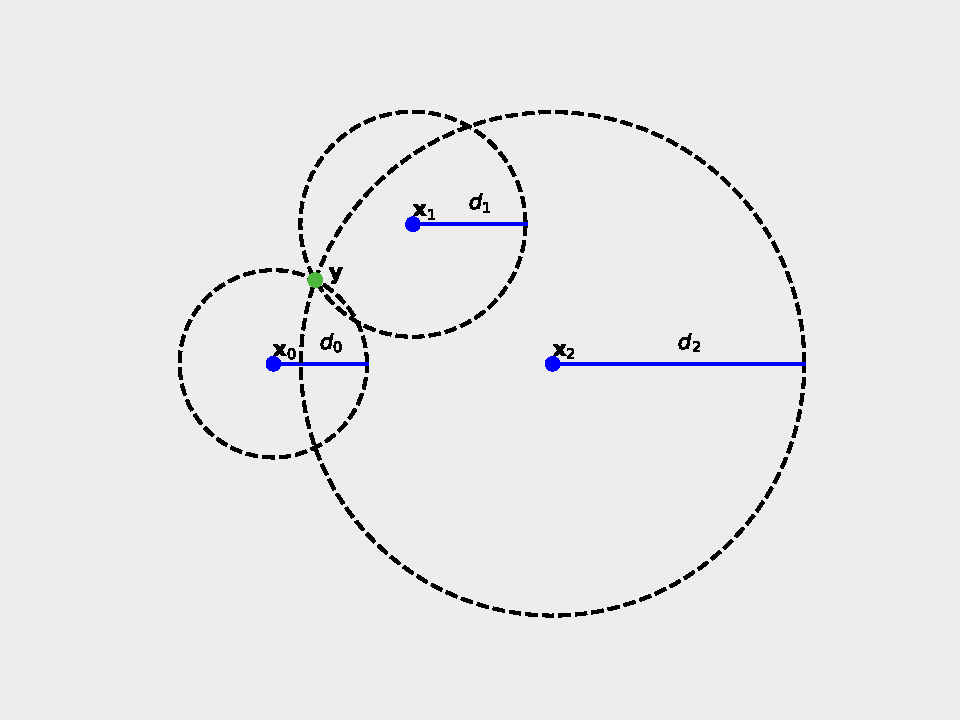
\includegraphics[width=.8\textwidth]{figs/trilateration_example.pdf}
  \caption{Position, $\mathbf{y}$, of entity determined by trilateration using known positions of $n = 3$ agents.}
  \label[fig]{trilat_example}
\end{figure}

\subsection{Coverage}\label[secc]{coverage}
As the goal of the swarm is to set up a network of agents in order to deliver precise positional data to entities entering the mission space,
it is clear from the previous section that three or more agents are needed to perform the task. Hence a point $\mathbf{y}\in\mathcal{F}$ is said
to be \textit{covered} iff. it is within communication range of at least three agents.

\subsection{Objective function derivation}\label[secc]{obj_formulation}
The objective function presented here is inspired by \cite{sun2014escaping}, but differs in that for the purpose of trilateration, it is required that at least three agents must be within
range of a point in order for the point to be covered.\newline
We assume we have a total of $N$ agents in a swarm $\mathcal{N}$ at our disposal. Furthermore it is assumed that all agents have homogenous local probability with respect to $r_{a}$:
\begin{equation}\label[eq]{homogenous_r}
  \begin{split}
    r_{a} &= r\;\forall\; a\in\mathcal{N}\\
    \tilde{V}(\mathbf{x}_{a}, \mathbf{y}) &= V(\mathbf{x}_{a}, \mathbf{y}, r)\\
    \tilde{p}(\mathbf{x}_{a}, \mathbf{y}) &= \hat{p}(\mathbf{x}_{a}, \mathbf{y}, r)
  \end{split}
\end{equation}
The probability of a point $\mathbf{y}$ being covered by $\mathcal{N}$ can now be expressed as:
\begin{equation}\label[eq]{cover_prob}
  \Phi^{3^{+}}_{\mathcal{N}}(\mathbf{y}) = 1 - \Phi^{0}_{\mathcal{N}}(\mathbf{y}) - \Phi^{1}_{\mathcal{N}}(\mathbf{y}) - \Phi^{2}_{\mathcal{N}}(\mathbf{y})
\end{equation}
In order to formulate a distributed optimization algorithm, we rewrite the coverage supplied by $\mathcal{N}$ with focus on a single drone $a$.
We partition the swarm, $\mathcal{N}$, into two disjoint sets: $\{a\}$ and $\mathcal{N}\setminus\{a\}$. Using this we can rewrite \eqref{cover_prob} as:
\begin{equation}\label[eq]{distr_cover_derivation}
  \begin{split}
    \Phi^{3^{+}}_{\mathcal{N}}(\mathbf{y}) &= 1\\
    &- \big(1-\tilde{p}(\mathbf{x}_{a}, \mathbf{y})\big)\prod_{k\in\mathcal{N}\setminus\{a\}}\big(1-\tilde{p}(\mathbf{x}_{k}, \mathbf{y}))\\
    &- \tilde{p}(\mathbf{x}_{a}, \mathbf{y})\prod_{k\in\mathcal{N}\setminus\{a\}}\big(1-\tilde{p}(\mathbf{x}_{k}, \mathbf{y}))\\
    &- \big(1-\tilde{p}(\mathbf{x}_{a}, \mathbf{y})\big)\sum_{j\in\mathcal{N}\setminus\{a\}}\tilde{p}(\mathbf{x}_{j}, \mathbf{y})\prod_{k\in\mathcal{N}\setminus\{a\}\setminus\{j\}}\big(1-\tilde{p}(\mathbf{x}_{k}, \mathbf{y})\big)\\
    &- \tilde{p}(\mathbf{x}_{a}, \mathbf{y})\sum_{j\in \mathcal{N}\setminus\{a\}}\tilde{p}(\mathbf{x}_{j}, \mathbf{y})\prod_{k\in\mathcal{N}\setminus\{a\}\setminus\{j\}}\big(1-\tilde{p}(\mathbf{x}_{k}, \mathbf{y})\big)\\
    &- \big(1-\tilde{p}(\mathbf{x}_{a}, \mathbf{y})\big)\sum_{\mathcal{A}\in Comb(\mathcal{N}\setminus\{a\}, 2)}\prod_{j\in\mathcal{A}}\tilde{p}(\mathbf{x}_{j}, \mathbf{y})\prod_{k\in\mathcal{N}\setminus\{a\}\setminus\mathcal{A}}\big(1-\tilde{p}(\mathbf{x}_{k}, \mathbf{y})\big)\\
    &= 1\\
    &- \prod_{k\in\mathcal{N}\setminus\{a\}}\big(1-\tilde{p}(\mathbf{x}_{k}, \mathbf{y}))\\
    &- \sum_{j\in\mathcal{N}\setminus\{a\}}\tilde{p}(\mathbf{x}_{j}, \mathbf{y})\prod_{k\in\mathcal{N}\setminus\{a\}\setminus\{j\}}\big(1-\tilde{p}(\mathbf{x}_{k}, \mathbf{y})\big)\\
    &- \big(1-\tilde{p}(\mathbf{x}_{a}, \mathbf{y})\big)\sum_{\mathcal{A}\in Comb(\mathcal{N}\setminus\{a\}, 2)}\prod_{j\in\mathcal{A}}\tilde{p}(\mathbf{x}_{j}, \mathbf{y})\prod_{k\in\mathcal{N}\setminus\{a\}\setminus\mathcal{A}}\big(1-\tilde{p}(\mathbf{x}_{k}, \mathbf{y})\big)\\
  \end{split}
\end{equation}
Applying \eqref{Phi_def} to \eqref{distr_cover_derivation} yields:
\begin{equation}
  \Phi^{3^{+}}_{\mathcal{N}}(\mathbf{y}) = 1 - \Phi^{0}_{\mathcal{N}\setminus\{a\}}(\mathbf{y}) - \Phi^{1}_{\mathcal{N}\setminus\{a\}}(\mathbf{y}) - \Phi^{2}_{\mathcal{N}\setminus\{a\}}(\mathbf{y})\big(1-\tilde{p}(\mathbf{x}_{a}, \mathbf{y})\big)
\end{equation}
From the viewpoint of agent $a$, the swarm can be partitioned into three disjoint sets: $\{a\}$, $\mathcal{B}_{a}$ and $\mathcal{C}_{a}$. The latter sets are defined as:
\begin{align}\label[eq]{neigh_def}
  \mathcal{B}_{a} &= \{j\in\mathcal{N}\setminus\{a\}: \norm{\mathbf{x}_{a}-\mathbf{x}_{j}} \leq r\}\\
  \mathcal{C}_{a} &= \{j\in\mathcal{N}\setminus\{a\}: \norm{\mathbf{x}_{a}-\mathbf{x}_{j}} > r\}
\end{align}
